\section{Standard Method in Itemset Mining}

After encoding the base constraints,
the subsequent step involves applying the standard method to encode formula \ref{eq:4}.

To solve the problem $q_1 + q_2 + ... + q_n \ge \lambda$, we can use the standard method known as $C_{n-k+1}$.

The fundamental idea behind this algorithm is as follows: Consider a set of $n$ elements.
If there are at least $k$ true elements, it is equivalent to having at most $n-k$ false elements.
In simpler terms, when selecting $n-k+1$ elements, there is a guarantee of having at least one true element among them.

% image
\begin{figure}[H]
    \centering
    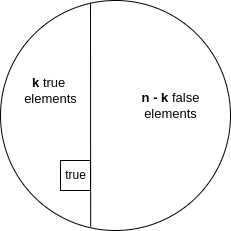
\includegraphics[width=0.38\textwidth]{chapter2/image/standard.png}
    \caption{Illustration of the standard method $C_{n-k+1}$}
    \label{fig:2_1}
\end{figure}

To illustrate this concept further, let's take an example where $n = 5$ and $\lambda = 3$.
In this scenario, we can employ the following constraint to depict the standard method

\begin{center}
    $q_1 + q_2 + q_3 + q_4 + q_5 \ge 3$
\end{center}

We can use the constraint below to represent the concept of having at least 3 true elements among 5 elements:
\begin{equation}
    \label{eq:5}
    \begin{aligned}
               & (q_1 \vee q_2 \vee q_3) \\
        \wedge & (q_1 \vee q_2 \vee q_4) \\
        \wedge & (q_1 \vee q_2 \vee q_5) \\
        \wedge & (q_1 \vee q_3 \vee q_4) \\
        \wedge & (q_1 \vee q_3 \vee q_5) \\
        \wedge & (q_1 \vee q_4 \vee q_5) \\
        \wedge & (q_2 \vee q_3 \vee q_4) \\
        \wedge & (q_2 \vee q_3 \vee q_5) \\
        \wedge & (q_2 \vee q_4 \vee q_5) \\
        \wedge & (q_3 \vee q_4 \vee q_5) \\
    \end{aligned}
\end{equation}

Then with $n$ elements and $\lambda$, we can present the constraint as:

\begin{equation}
    \label{eq:6}
    \begin{aligned}
         & \bigwedge_{i=1}^{n-\lambda+1} \left( \bigvee_{j=i}^{i+\lambda-1} q_j \right) \\
    \end{aligned}
\end{equation}

In this equation, the outer conjunction $\bigwedge$ iterates from $i=1$ to $n-\lambda+1$, representing the range of possible starting positions for the subsequence of length $\lambda$. The inner disjunction $\bigvee$ iterates from $j=i$ to $i+\lambda-1$, representing the elements within each subsequence. By combining these subsequence constraints with the conjunction operator, we ensure that at least one subsequence of length $\lambda$ contains all true elements.

This constraint, along with the previously mentioned constraints \ref{eq:2}, \ref{eq:3}, and \ref{eq:6}, can be used to resolve the problem of Itemset Mining.
